\documentclass[../primer.tex]{subfiles}

\begin{document}

% --------------------------------------------------
\chapter{A Demonstration}
% --------------------------------------------------
(Here we give a tour of UQ through an example; a la Saltelli's Primer.)

\section{Buoyancy-Driven Cavity Flow}
% --------------------------------------------------
Here we consider the buoyancy-driven cavity flow of a viscous fluid, pictured
schematically in Figure \ref{fig:cavity-schematic}.\footnote{This example was
  originally prepared by Dr. Gary Tang.} This is a model problem for studying
the effects of uncertainties in fluid properties on buoyancy-driven flows, with
an eye towards quantifying the uncertainties in climate modeling.

\begin{figure}[!ht]
  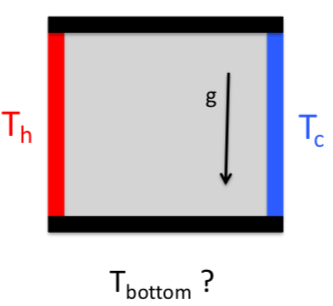
\includegraphics[width=0.75\textwidth]{./images/cavity_schematic}
  \caption{Schematic of density-driven cavity flow. The density of the fluid
    decreases with increasing temperature, and the walls are held at constant
    hot $T_h$ and cold $T_c$ temperatures. The resulting density gradients lead
    to an instability, which in turn drive fluid flow. The quantity we are
    interested in here is the temperature of the bottom wall.}
  \label{fig:cavity-schematic}
\end{figure}

\begin{figure}[!ht]
  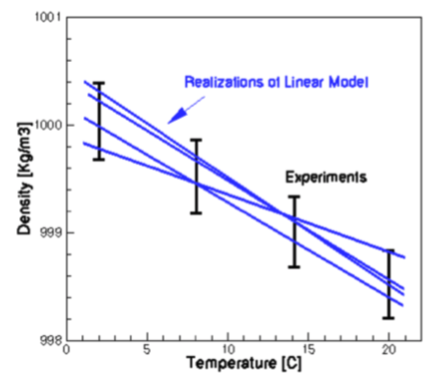
\includegraphics[width=0.75\textwidth]{./images/density_linear}
  \caption{Experimental intervals for temperature-density relation of cavity
    fluid. The data are compatible with a linear relationship, so we assume a
    family of linear models for the equation of state (EOS) -- informed by the
    data -- for uncertainty propagation.}
  \label{fig:density-linear}
\end{figure}

\begin{figure}[!ht]
  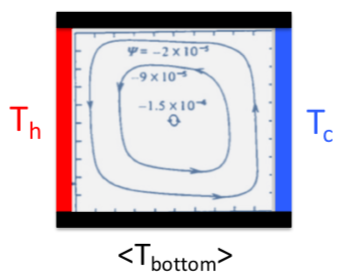
\includegraphics[width=0.80\textwidth]{./images/cavity_single}
  \caption{Mean streamfunction contours using the linear EOS assumption. These
    results show a single recirculation driving flow upward near the hot wall,
    and falling near the cold wall. (TODO: Re-generate; flip arrows)}
  \label{fig:cavity-schematic}
\end{figure}

\begin{figure}[!ht]
  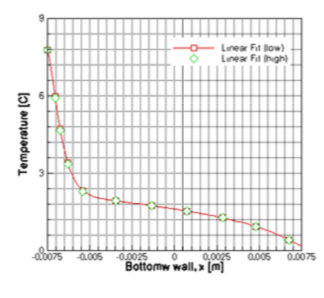
\includegraphics[width=0.75\textwidth]{./images/bot_wall_single}
  \caption{Bounds of bottom-wall behavior over all EOS models considered. Note
    that all the curves collapse. All the conditions considered result in
    \emph{the same} recirculation -- the uncertainty in our qoi is zero! This
    should seem fishy -- we will investigate further below.}
  \label{fig:bot-wall-single}
\end{figure}

\begin{figure}[!ht]
  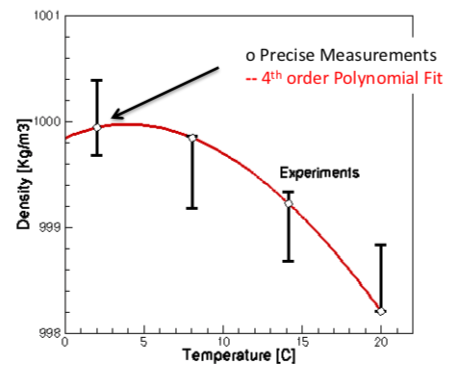
\includegraphics[width=0.75\textwidth]{./images/density_poly}
  \caption{Experimental intervals \emph{and point estimates} for
    temperature-density relation of cavity fluid -- the fluid is water, which
    undergoes a density inversion near freezing conditions! This slight
    nonlinearity has important ramifications for the flow field, which we
    consider in Figure \ref{fig:cavity-double}.}
  \label{fig:density-poly}
\end{figure}

\begin{figure}[!ht]
  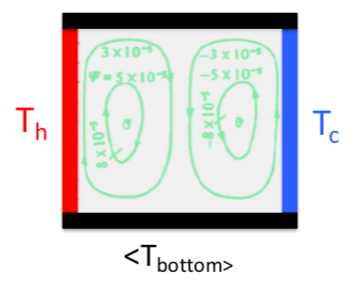
\includegraphics[width=0.75\textwidth]{./images/cavity_double}
  \caption{Streamfunction contours using the (single) polynomial EOS fit. These
    results show a pair of recirculation regions, which change the qualitative
    behavior significantly.}
  \label{fig:cavity-double}
\end{figure}

\begin{figure}[!ht]
  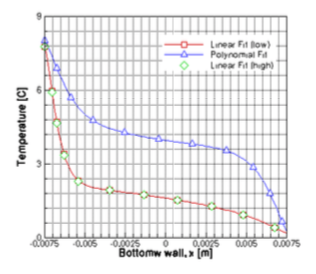
\includegraphics[width=0.75\textwidth]{./images/bot_wall_double}
  \caption{Bounds of bottom-wall behavior over all linear EOS models, and using
    the polynomial fit. We can see that the double-recirculation results in a
    considerably higher bottom-wall temperature -- hot fluid is transported to
    the middle of the bottom-wall via the double-recirculation, resulting in a
    generally hotter temprature profile.}
  \label{fig:bot-wall-double}
\end{figure}

\begin{figure}[!ht]
  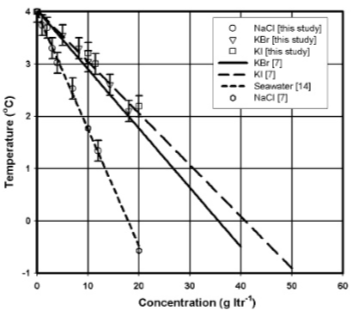
\includegraphics[width=0.75\textwidth]{./images/inversion_salt}
  \caption{Point of density inversion for water at different salinity
    concentrations.}
  \label{fig:inversion-salt}
\end{figure}

\end{document}
